\section{$G_2$: definitions and properties}
\label{sec:g2def}

Let's move on to the modular forms on $G_2$.
First, we need to understand about the group $G_2$.
In short:
\begin{center}
\text{$G_2$ is an \emph{automorphism group of octonions.}}
\end{center}
You may have heard about the word octonion, but not the definition itself (I didn't know the actual definition until I read about $G_2$).
First of all, over $\mathbb{R}$, we have \emph{two} octonions: split one and non-split one.
These two give two different $G_2$: split $G_2$ and non-split/compact $G_2$.
You can consider them as an analogue of $\rM_2(\mathbb{R})$ vs Hamilton's quaternion.
In this note, we will only consider \emph{split} octonions and \emph{split} $G_2$, and modular forms on it.
The main reference is Baez's article on octonions \cite{baez2002octonions}.

\subsection{Split octonion}

The split octonion, which we denote as $\bO$, was first constructed by Cayley and Dickson.
As a set, it is just two copies of Hamilton's $\mathbb{H}$.
We define a multiplication of two pairs as:
$$
(a, b) \cdot (c, d) = (ac + \bar{d}b, da + b\bar{c}).
$$
$(1, 0)$ becomes an identity.
This multiplication is not even associative; but still form a \emph{composition algebra}: it admits a multiplicative quadratic norm.
We first define a conjugate of an element as
$$
(a, b)^\ast = (\bar{a}, -b)
$$
and the norm is defined by $\rN(x) = x^\ast x$.
If we write the elements of $\bH$ in a usual way, $a = a_0 + a_1 i + a_2 j + a_3 k$ and $b = b_0 + b_1 i + b_2 j + b_3 k$, then the norm $\rN((a, b))$ becomes
\begin{align*}
    \rN((a, b)) = (a_0^2 + a_1^2 + a_2^2 + a_3^2) - (b_0^2 + b_1^2 + b_2^2 + b_3^2).
\end{align*}
Especially, it gives a quadratic form of a signature $(4, 4)$.
We can decompose an arbitrary element as a sum of the ``real part'' and the ``imaginary part'': $(a, b) = a_0(1, 0) + (a - a_0, b)$.
Then the trace of an element becomes $\Tr((a, b)) = (a, b) + (a, b)^\ast = 2a_0 (1, 0)$.
We will denote the space of purely imaginary octonions (i.e. $a_0 = 0$) by $\Im(\bO)$, which is orthogonal to $\Re(\bO) \simeq \mathbb{R}$.
Note that we have a trilinear form on $\bO$, given by
$$
\bO \times \bO \times \bO \to \bR, \,\, (x, y, z) \mapsto \Tr((xy)z)
$$
(we have $\Tr((xy)z) = \Tr(x(yz))$, even if the multiplication is not associative).

\subsection{Definition and dimension}
\label{subsec:g2def}

Now, let us get back to the definition.
$G_2$ is an automorphism group of $\bO$:
$$
G_2 = \Aut(\bO) = \{g \in \GL(\bO): g(x\cdot y) = (gx) \cdot (gy) \,\,\forall x, y \in \bO\}.
$$
Then any $g \in G_2$ also preserves conjugations, norms and inner products.
Especially, we have an embedding $G_2 \hookrightarrow \SO(4, 4)$.
We can do slightly better: $\Im(\bO)$ is stable under $G_2$, and we get $G_2 \hookrightarrow \SO(3, 4)$.
Thus, we get a 7-dimensional faithful representation of $G_2$, which is in fact the smallest irreducible representation of $G_2$.

What is the dimension of $G_2$? Since it sits inside $\SO(3, 4)$, we have an upper bound $\dim \SO(3, 4) = \binom{8}{2} = 28$.
In fact, the actual dimension is exactly half of it:

\begin{proposition}
\label{prop:dim}
$\dim G_2 = 14$.
\end{proposition}

\begin{proof}
Each element $g \in G_2$ is completely determined by its image of a \emph{basic triple} $\{e_1, e_2, e_3\}$, that is, the set of orthonormal generators $\bO$: $\rN(e_1) = \rN(e_2) = \rN(e_3) = 1$, and $\langle e_i, e_j \rangle = 0$ for all $i \ne j$.
They generate $\bO$ in the sense that $\{1, e_1, e_2, e_3, e_1 e_2, e_2 e_3, e_3 e_1, e_1 e_2 e_3\}$ becomes a $\bR$-basis of $\bO$.
Now, consider how many ``choices'' we have for $e_1' = ge_1, e_2' = ge_2, e_3' = ge_3$:
\begin{enumerate}
    \item $e_1'$ is a purely imaginary element of norm 1, so it is a codimenion 1 space of $\Im(\bO) \simeq \bR^7$, hence dimension is 6.
    \item $e_2'$ is a norm 1 element in $\Span(1, e_1)^\perp \simeq \bR^6$, hence the dimension is $6 -1 = 5$.
    \item $e_3'$ is a norm 1 element in $\Span (1, e_1, e_2, e_1 e_2)^\perp \simeq \bR^4$, hence the dimension is $4 - 1 = 3$.
\end{enumerate}
Thus, we get $\dim G_2 = 6 + 5 + 3 = 14$.
\end{proof}

\subsection{Lie algebra $\frg_2$}

Let's move on to the semisimple Lie algebra $\frg_2 = \Lie(G_2)$.
Instead of giving detailed proofs of the known facts on $\frg_2$, we will start with the Dynkin diagram of $\frg_2$ and see what we can say about $\frg_2$ from it.
Here is the tiny little cute Dynkin diagram of $\frg_2$:
$$
\dynkin G2
$$
Now, let us see what this diagram tells us about $\frg_2$.
First of all, we have two vertices, so the rank of $\frg_2$ is 2 and there are two simple roots.
In addition, there are three lines between two vertices, which tell us the angle between the simple roots and the length ratio: the angle is $5\pi / 6$, where the ratio between the lengths of the simple roots is $\sqrt{3}$.
Let's call the longer one (resp. the shorter one) as $\alpha$ (resp. $\alpha'$).


\begin{center}
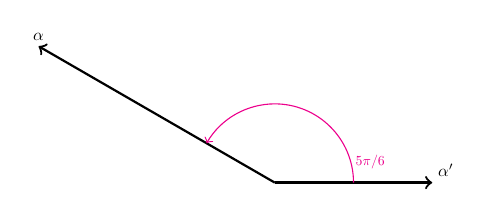
\begin{tikzpicture}

\draw[->,black!80!black,thick] (0,0) -- (0:2cm);
\draw[->,black!80!black,thick] (0,0) -- (150:3.464cm);
\draw[magenta,->](1,0) arc(0:150:1cm)node[pos=0.1,right,scale=0.5]{$5\pi/6$};
\node[anchor=south west,scale=0.6] at (2,0) {$\alpha'$};
\node[anchor=south,scale=0.6] at (-3, 1.732) {$\alpha$};
\end{tikzpicture}
\end{center}
By taking suitable $\bZ$-linear combinations, we can build more roots out of these simple roots:

\begin{center}
\begin{tikzpicture}
\foreach\ang in {60,120,...,360}{
 \draw[->,black!80!black,thick] (0,0) -- (\ang:2cm);
}
\foreach\ang in {30,90,...,330}{
 \draw[->,black!80!black,thick] (0,0) -- (\ang:3.464cm);
}
\draw[magenta,->](1,0) arc(0:150:1cm)node[pos=0.1,right,scale=0.5]{$5\pi/6$};
\node[anchor=south west,scale=0.6] at (2,0) {$\alpha'$};
\node[anchor=south,scale=0.6] at (-3, 1.732) {$\alpha$};
\node[anchor=south,scale=0.6] at (-1, 1.732) {$\alpha + \alpha'$};
\node[anchor=south,scale=0.6] at (1, 1.732) {$\alpha + 2 \alpha'$};
\node[anchor=south,scale=0.6] at (3, 1.732) {$\alpha + 3 \alpha'$};
\node[anchor=south,scale=0.6] at (0, 3.464) {$2\alpha + 3 \alpha'$};
\draw [dashed] (-6.464, 1.732) -- (6.464, -1.732);
\end{tikzpicture}
\end{center}
Recall that the only possible degrees between two root vectors are multiples of $\pi/6$, and no scaled vectors of given roots other than the vector and its opposite can appear as roots (reduced).
The ones above the dashed line (i.e. ones with names) are the chosen positive roots.
This gives the root space decomposition of $\frg_2$, where we can find the dimension of $\frg_2$ (hence Proposition \ref{prop:dim}) from this:
$$
\dim \frg_2 = \text{(rank)} + \text{(number of roots)} = 2 + 12 = 14.
$$
The highest root is $\beta_0 = 2 \alpha + 3 \alpha'$ (literally the ``highest'' one in the above diagram), and the Weyl group of $\frg_2$ is the symmetric group of a regular hexagon, which is the dihedral group of order 12.


\subsection{$G_2$ as a symmetry group of rolling balls}

Here we introduce an another definition of $G_2$, as a symmetry group of \emph{rolling balls}, discovered by Baez and Huerta \cite{baez2014g2}.
This section is not necessary for the upcoming discussions on modular forms\footnote{Maybe related? Who knows!}, but we include this because of its own interest.

We have a large ball of radius $R > 1$, and we are going to roll a unit ball around it, without slipping or twisting.
Then the corresponding configuration space is $\bS^2 \times \SO(3)$: $\bS^2$ for the point of contact and $\SO(3)$ for the rotation of the small ball.
Now, we define ``lines'' on the configuration space as paths along a great circle on the large ball, i.e. two points are connected if one can move the small ball from one state to the other state by rolling over a great circle (without slipping or twisting, of course).

Now, we consider another (incidence) geometry, comes from our one and only\footnote{Of course, there are two, but let's focus on the split one. Sorry for the non-split octonion...} octonion $\bO$.
The ``points'' are 1-dimensional \emph{null subalgebra} of $\Im(\bO)$: $p_x := \langle x \rangle \subset \Im(\bO)$ with $\rN(x) = 0$.
The ``lines'' are 2-dimensional null subalgebras spanned: i.e. two points $p_x = \langle x \rangle$ and $p_y = \langle y \rangle$ are connected if and only if $xy = 0 = yx$.
Then the group $G_2$ acts naturally on this space, which we denote as
$$
\mathbb{P}C = \{\langle x \rangle: 0 \ne x \in \Im(\bO), \rN(x) = 0\}.
$$
One can check that this space is isomorphic to
$$
\frac{\bS^2 \times \bS^3}{(a, b) \sim (-a, -b)} \simeq \mathbb{RP}^{2} \times \bS^3
$$
which is very close to the configuration space of the rolling ball, but not exactly.
To make them coincide, we can replace
\begin{itemize}
    \item small unit ball with \emph{spinor}: it needs to roll \emph{twice} to get back to the original position
    \item large ball with $\mathbb{RP}^{2}$: in other words, rolling a pair of spinor together in sync around the large ball.
\end{itemize}
Now we have the following amazing theorem.
\begin{theorem}[Baez--Huerta \cite{baez2014g2}]
    The symmetry group of a rolling spinor over $\mathbb{RP}^2$ is $G_2$ if and only if $R = 3$.
\end{theorem}